\section{Introduction}
\label{sec:intro}

Understanding long videos presents fundamental challenges due to complex temporal dependencies and varying information granularity. 
Recent approaches~\cite{liu2025videomind,pan2025timesearch} typically adopt a two-stage framework: first localizing relevant temporal segments, then reasoning over the retrieved content. This retrieval-then-reasoning paradigm offers a structured and interpretable framework for tackling intricate video understanding tasks.

However, existing grounding models perform unsatisfactorily, 
often struggling to generalize across diverse video domains~\cite{shi2024aotd}.
In this context, we advocate for developing a universal temporal grounding model, that is capable of accommodating videos across a wide range of viewpoints~(egocentric and exocentric perspectives), topics~(from cooking and daily activities to sports, movies, and games), and durations~(from brief clips to multi-hour videos). Such universality is crucial for real-world deployment, where video data is inherently heterogeneous and user queries are highly diverse.


\begin{figure*}[t]
    \centering
    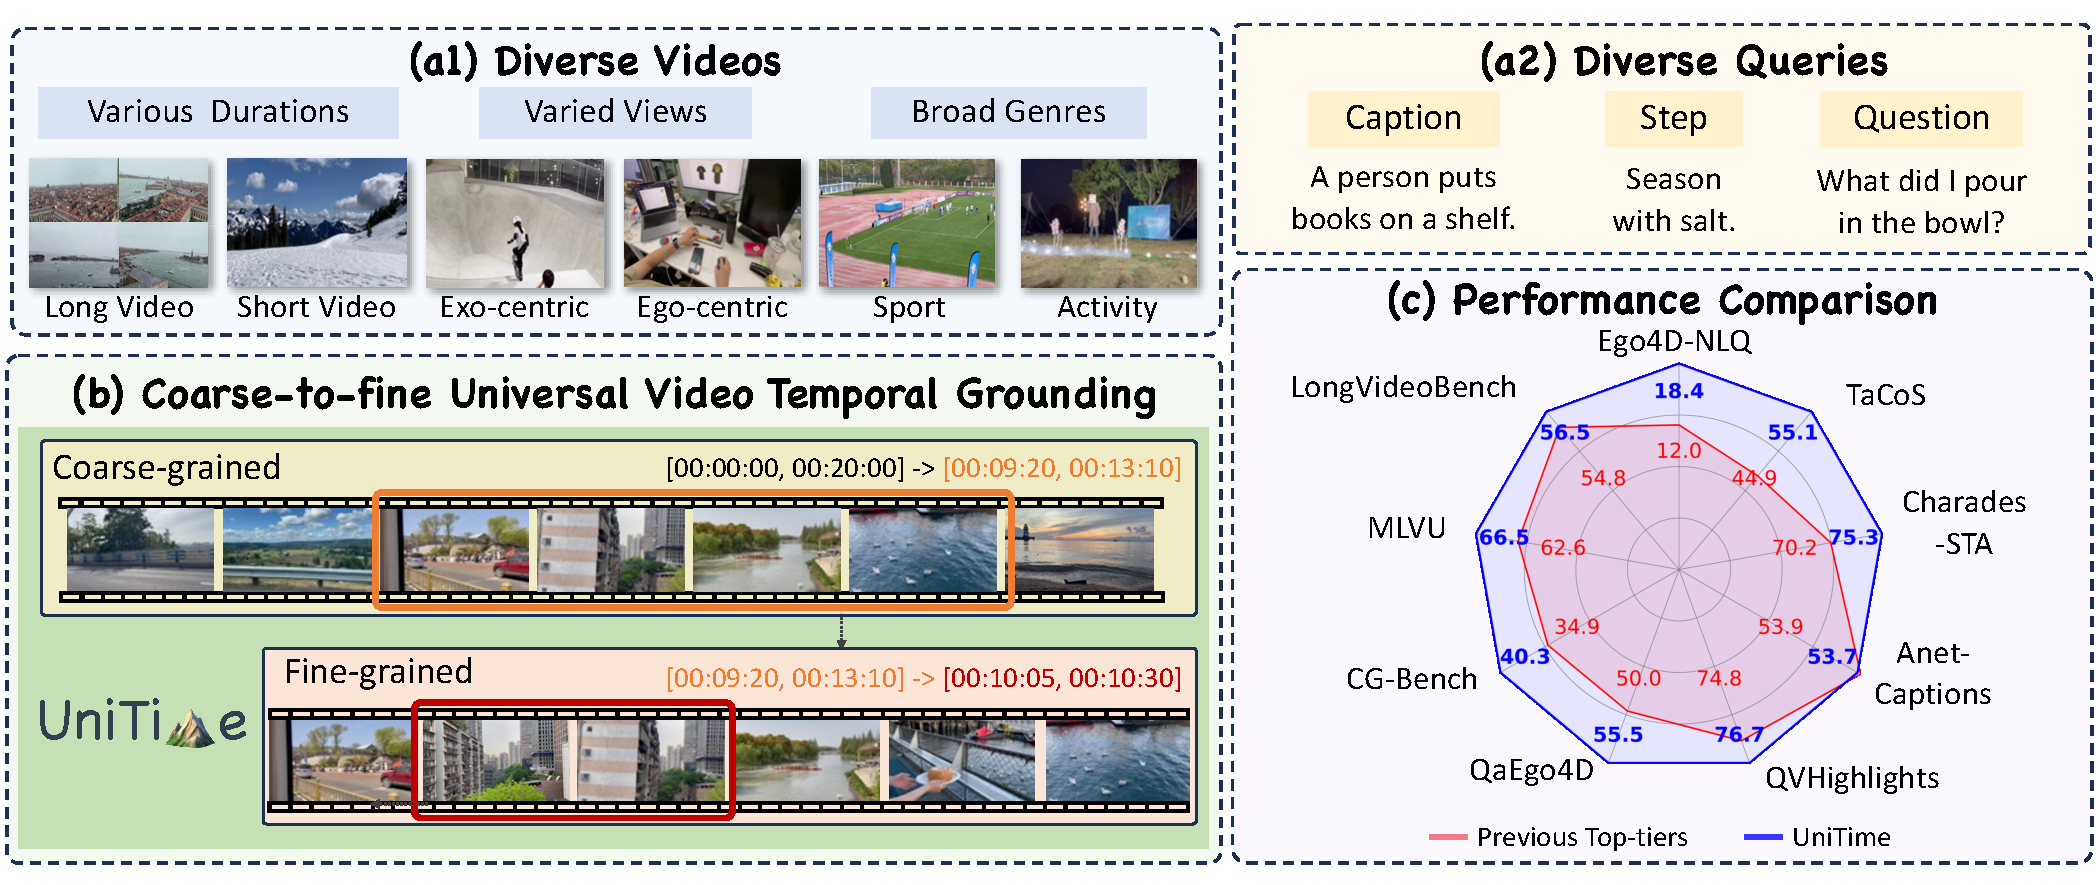
\includegraphics[width=\linewidth]{img/teaser_arxiv.pdf}
    \captionof{figure}{The \textbf{\Model{}} framework empowers MLLMs with advanced universal temporal grounding capabilities.
    (a) \Model{} can handle diverse videos with various views, genres, and durations, as well as comprehend complex language queries.
    (b) \Model{} achieves universal temporal grounding through a coarse-to-fine approach.
    (c) Performance comparison on temporal grounding and video question answering benchmarks demonstrates the superior capabilities of \Model{}.}
    \label{fig:teaser}
    \vspace{-10pt}
\end{figure*}

Research on temporal grounding falls into two paradigms. 
The first includes discriminative or dual-encoder-based approaches~\cite{carion2020end,lei2021detecting}, which typically rely on dataset-specific fine-tuning and lightweight architectures, such as DETR-like frameworks. While computationally efficient, these models often struggle to generalize to unseen content due to limited language encoding capabilities, hindering the understanding of complex or user-driven queries, and constrained visual representations.
In contrast, recent work leverages Multi-modal Large Language Models (MLLMs)~\cite{meinardus2024surprising,zeng2024timesuite}, which excel at language understanding and demonstrate promising results on video temporal grounding. However, their applicability to long videos is hindered by short context windows and high memory demands, making them impractical for processing video inputs spanning tens of thousands of tokens.

In this paper, we further explore the potential of MLLMs towards universal temporal grounding in videos.
Our proposed model, termed as \textbf{\Model{}}, encodes temporal information by interleaving timestamp tokens with video tokens, 
enabling precise boundary generation for natural language queries.
To handle videos of varying lengths, we introduce an adaptive frame scaling mechanism that adjusts temporal and spatial granularity based on video duration. Specifically, for long videos, the model can be adopted for multi-stage inference-time computation: 
initial coarse-grained sampling enables segment-level grounding, followed by fine-grained sampling within candidate regions to refine boundaries. This iterative process progressively improves grounding precision. 
To improve training efficiency, we adopt a video-centric training paradigm that concatenates multiple queries and their corresponding segments per video, allowing the model to process them in a single pass. This minimizes the computational overhead of autoregressive decoding over repeated video tokens.

To rigorously evaluate efficacy, 
we pre-train \textbf{\Model{}} on diverse, high-quality temporally grounded video datasets and assess its performance on two key tasks: 
\textbf{temporal grounding} (in both zero-shot and fine-tuning settings) and downstream \textbf{video question answering}~(VideoQA) for long videos. 
For temporal grounding, we conduct experiments on two long-video and three short-video benchmarks, where our model consistently outperforms existing methods in both straightforward and complex retrieval scenarios. 
For downstream VideoQA, we evaluate on four widely used long-video benchmarks using a retrieval-augmented protocol: first, our framework localizes the relevant video segment; then, an off-the-shelf VideoQA model answers the query based on the localized segment. Compared to prior approaches, our method demonstrates superior generalization, delivering more accurate and comprehensive video understanding, especially for long videos.

% The remainder of the paper is organized as follows: 
% Section~\ref{sec:method} formally defines the temporal grounding task and describes our proposed method in detail, including its model architecture, training strategies, and the key innovations that distinguish our approach from existing methods.
% Section~\ref{sec_exp} presents comprehensive experimental results, including ablation studies and comparisons with state-of-the-art methods, to thoroughly validate the effectiveness and robustness of our approach across multiple benchmarks.
% Section~\ref{sec:related} provides an overview of the relevant literature. Overall, our method achieves improved performance on both temporal grounding and long-video VideoQA benchmarks.

The remainder of the paper is organized as follows: 
Section~\ref{sec:method} formulates the temporal grounding task and details our proposed method.
Section~\ref{sec_exp} presents ablation studies and comparisons to validate our approach. 
Section~\ref{sec:related} provides an overview of the relevant literature.
Overall, our method achieves improved performance on both temporal grounding and long-video VideoQA benchmarks.